\section{Background}
\noindent This section overviews important information and concepts in physics engines, which are relevant to their usage in CAV simulations. 
Particularly, on how physics engines operate and the sources of non-determinism in these engines necessary to understand the contribution of this paper.
\subsection{Overview of a Game Loop}\label{GameLoopSection}
\noindent The game loop is responsible for the interaction between the math, physics and rendering engines\cite{GameEngineArchBook}.
Figure \ref{GameEngineLoopDiagram} depicts a very basic diagram showing the flow in a game loop. 
A traditional game loop is broken up into three distinct phases: processing the inputs, updating the game world (Physics Engine), and generating outputs (Rendering).
\begin{figure}[h]
\centering
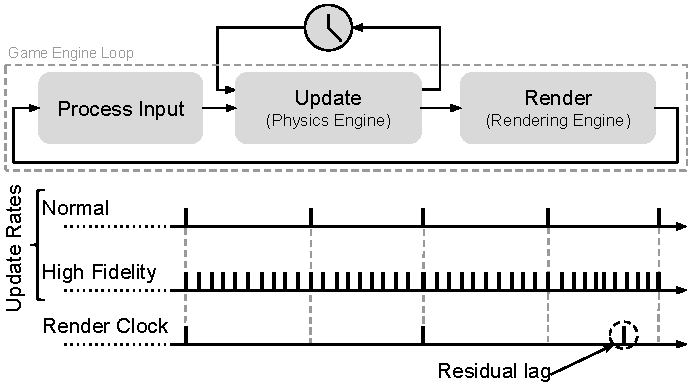
\includegraphics[width=0.5\textwidth]{Other/Figures/GameEngineLoop.pdf}
\caption{Game engine loop block diagram}
\label{GameEngineLoopDiagram}
\end{figure}
The first part of the game loop is to process the user input. Then comes update, which advances the AI and physics engine. Finally the rendering engine draws the game\cite{GameProgPatternsBook}.
It is crucial for this paper to understand how the rendering and physics engines operate together.
Briefly, the game loop operates as follows:\cite{GameProgPatternsBook} (see Figure \ref{GameEngineLoopDiagram})
\begin{itemize}[leftmargin=*]
    \item At the beginning of each tick (frame), the lag between the game clock and the real world is updated based on how much real time passed. This measures how far the game's clock is behind compared to the real world.
    \item Then the user inputs are processed.
    \item There is then an inner loop to update the physics engine, one fixed step at a time until it catches up with the real world. 
    The physics engine uses a fixed time step, because it makes everything simpler and more stable for physics and AI. 
    The shorter this fixed time step is, the more processing time it takes to catch up to real time and the more deterministic the engine becomes and vice versa\cite{GameEngineArchBook}\cite{GameProgPatternsBook}, as will be explained in section \ref{nondeterminisimSources}. 
    Thus, ideally the time step should be as short as possible, so that simulations run with high fidelity on fast machines. 
    However, if the fixed time step is too short i.e. less than the time it takes to process an ``Update" inner loop on some (slow) machines, then the simulation will simply never catch up on these slow machines.
    \item Rendering occurs once the physics engine catches up. The process then starts again.
\end{itemize} 

\noindent This process allows a game to simulate across a range of hardware, but the rendering will become of jerky quality on slower machines. \\\\
These engines update at fixed intervals and render whenever they can, which is not steady. 
This results in what is so called residual lag\cite{GameEngineArchBook}\cite{GameProgPatternsBook}, where the engine is trying to render between two consecutive updates. 
In this case, the engine will use extrapolation techniques to give a rough estimate of where it thinks the object should be. 
This often is sufficient for gaming purposes and unnoticeable to the user, in fact it improves the stuttery motion.
\subsection{Sources of non-determinism}\label{nondeterminisimSources}
\noindent After establishing an understanding of how physics engines work, the focus will now be on what causes these engines to be non-deterministic. 
The main reasons that could cause non-determinism are discussed below. \\\\
\noindent\underline{\textit{Floating Points:}}
A generic issue with computers are floating points precision. 
Various errors occur when doing arithmetic manipulations using floating points, especially when operating between large and small numbers due to rounding, memory limitations and so forth.\cite{FloatingPointArithmeticArticle}\cite{FloatingPointsBook}. 
Translating to the usage of CAV simulations for V\&V in physics engines, this could result in many precision issues resulting in complex non deterministic behaviours.\\\\ 
\noindent For instance, consider a simulation where the world is infinite and progressively  generated in the physics engine. 
After a few hundred meters, precision issues will start to occur, and will get progressively worse the further from the origin the simulation gets. 
This is due to the values of the coordinates being used in calculations are getting bigger and hence will not cope with small values that are critical for V\&V testing purposes. 
A solution to this problem is perhaps every time the simulations moves 100 meters away from the origin the entire world will move by 100m in the opposite direction. Thus, avoiding getting into floating point issues.\cite{FloatingPointArithmeticArticle}\\\\
\noindent There are many scenarios that could be addressed, and solutions to them will entirely depend on the characteristics of that specific scenario. There is no generalised solution for the floating problem, regardless of how good computers get there will always be a limitation. However, floating points as they stand could just be sufficient for V\&V testing purposes. Whenever they are not, smart solutions can be found to accommodate for these limitations.\\\\
\noindent\underline{\textit{Navigation meshes and AI:}}
Some CAV simulator developers claim that the built-in physics engines' AI is non-deterministic\cite{CARLABenchmark}. 
The validity of this depends on what are the built in AI algorithms being used by the engine. 
Most of them tend to use the A* algorithm\cite{AStarBook}, which is an algorithm with deterministic behaviour if the environment is deterministic\cite{AirsimUnrealArticle}\cite{UnrealAIDocumentation}. 
Therefore the determinism of the AI depends on the determinism of the engine and how its navigation meshes are created or modelled. It is interesting to note that changes can occur to meshes every time the simulation is loaded. This is mainly resorted to the different scheduling of threads. \\\\
\noindent\underline{\textit{Physics and Rendering clocks:}}
The inherent way of how these physics engines operate (i.e.game loops) causes the engine to be non-deterministic. 
A follow up from section \ref{GameLoopSection}, these engines use a variable frame rate, which is good for hardware scalability but creates a challenge for the physics engine which works best with small fixed time steps. 
The problem of having a variable frame rate could also be a reason for the non-deterministic behaviour of these engines. This issue could perhaps be of negligible significance if the time steps are small enough. \\

\noindent\underline{\textit{Scheduling of threads:}} Scheduling of threads is believed to be the main reason for the non deterministic behaviour of these engines. Given the same hardware the output should always be the same, unless scheduling of the threads change, this would then cause non-deterministic behaviours. To solve this one would have to control all of the threads, which is a very involved and to achieve that one would need to replace or control the whole run-time system to allocate the same threads in the same order.

